\documentclass[compress]{beamer}

\usetheme{Antibes}
\usepackage{bclogo}
\usepackage{framed}
%---------------------------------------------------------------------------------- 
\newenvironment {gbar}[1]{ %
	\def \FrameCommand {{\color {#1}\vrule width 2pt}\colorbox {gray!20}} %
	\MakeFramed {\advance\hsize -\width  \FrameRestore }} %
{\endMakeFramed}
%---------------------------------------------------------------------------------- 
\usepackage[style=authoryear,url=false,isbn=false,backend=biber,doi=false]{biblatex}
\addbibresource{mybib.bib}
\setbeamercolor{structure}{fg=red!60!black}
\setbeamercolor{block title}{bg=black}
\setbeamercolor{frametitle}{bg=white,fg=black}
\useinnertheme{circles}
\usepackage{booktabs}
\usepackage[most]{tcolorbox}
\usepackage{emojione}
\usepackage{soul}

\usepackage{fontspec}
\setsansfont{Linux Biolinum O}
\newcommand{\at}{\makeatletter @\makeatother}
\usepackage[absolute,overlay]{textpos}
\setlength{\TPHorizModule}{\paperwidth}
\setlength{\TPVertModule}{\paperheight}
\graphicspath{{F:/Official/Talks/Hypophosphatemia/osteomalacia/}}
%----------------------------------------------------------------------------------
\setbeamertemplate{navigation symbols}{} 
%---------------------------------------------------------------------------------- 
\setbeamercolor{bibliography entry author} {fg=black!70}
\setbeamercolor{bibliography entry title} {fg=black!70}
\setbeamercolor{bibliography entry location} {fg=black!70}
\setbeamercolor{bibliography entry note} {fg=black!70}
\newcommand*\myitem{%
	\item[\color{teal!60!black}\scalebox{0.9}{\textbullet}]}
\setbeamerfont{footnote}{size=\scriptsize}
\usepackage{tikz}
 \renewcommand\arraystretch{1.3}
 \newcommand{\myred}[1]{\textcolor{red!60!black}{#1}}
 %---------------------------------------------------------------------------------- 
\tikzset{
	treenode/.style = {shape=rectangle, rounded corners,
		draw, align=center,
		top color=white, bottom color=blue!20},
	root/.style     = {treenode, bottom color=purple!40},
	env/.style      = {treenode, font=\scriptsize},
	dummy/.style    = {circle,draw}
}
 
%----------------------------------------------------------------------------------
\author[Karthik]{Karthik Balachandran}
\title{Hypophosphatemia}
\subtitle{Approach in India}
\date{}
\institute[SRMC]{Sri Ramachandra Medical College \\ Chennai}
%----------------------------------------------------------------------------------

\begin{document}

\begin{frame}[plain]
	\maketitle
\end{frame}

%----------------------------------------------------------------------------------
\section{Background}
%---------------------------------------------------------------------------------- 
%---------------------------------------------------------------------------------- 
\begin{frame}{Hypophosphatemia }
\begin{block}{Definition}
	Serum phosphate $<$ 2.5 mg/dl
\end{block}
\pause
\begin{bclogo} [logo=\bcattention,barre=none,noborder=true]{Beware}
	\begin{gbar} {teal}
		Infants have higher values.\\
		$ \therefore Normal \implies Abnormality $
	\end{gbar}
\end{bclogo}

\end{frame}
%----------------------------------------------------------------------------------

\begin{frame}{ Hypophosphatemia -Severity }
	  \begin{description}[Moderate]
		\item[Mild]  $2 - 2.5 mg/dl $
		\item[Moderate]  $ 1- 2 mg/dl $
		\item[Severe]  $ < 1 mg/dl $
	\end{description}
\end{frame}
%----------------------------------------------------------------------------------
\begin{frame}{ Epidemiology }
	\begin{itemize}
		\item Upto 5\% of hospitalized patients 
		\item 0.5\% of them severe
		\item Chronic hypophosphatemia - limited data
	\end{itemize}
\end{frame} 
%----------------------------------------------------------------------------------

%---------------------------------------------------------------------------------- 
\section{Phosphate biology}
\begin{frame}{How is phosphate regulated\footfullcite{Torres.2011}?  }
	\begin{center}
		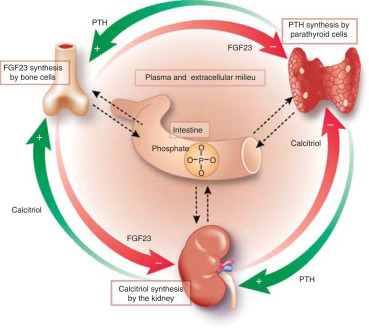
\includegraphics[scale=0.7]{physiology.jpg}
	\end{center}
	
\end{frame} 
%---------------------------------------------------------------------------------- 
%----------------------------------------------------------------------------------
\begin{frame}[fragile]{Penrose Triangle of hormones  }
 	\begin{center}
 			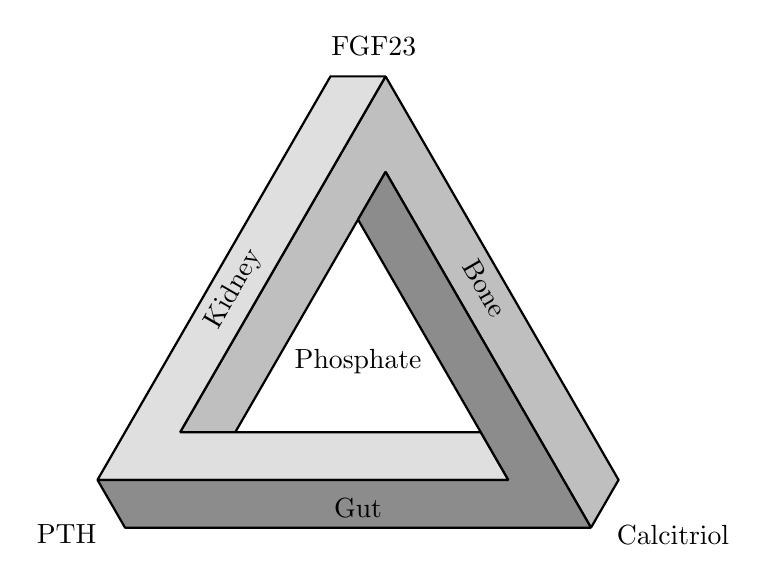
\begin{tikzpicture}[scale=1, line join=bevel]
 		
 		% \a and \b are two macros defining characteristic
 		% dimensions of the Penrose triangle.       
 		\pgfmathsetmacro{\a}{1.8}
 		\pgfmathsetmacro{\b}{0.7}
 		
 		\tikzset{%
 			apply style/.code     = {\tikzset{#1}},
 			triangle_edges/.style = {thick,draw=black}
 		}
 		
 		\foreach \theta/\facestyle/\city/\al\/\ang in {%
 			0/{triangle_edges, fill = gray!50}/Bone/below/-60,
 			120/{triangle_edges, fill = gray!25}/Kidney/below/60,
 			240/{triangle_edges, fill = gray!90}/Gut/above/0}
 		{
 			\begin{scope}[rotate=\theta]
 			\draw[apply style/.expand once=\facestyle]
 			({-sqrt(3)/2*\a},{-0.5*\a})                   --
 			++  (-\b,0)                                   --
 			({0.5*\b},{\a+3*sqrt(3)/2*\b})                --node[\al,rotate=\ang]{\city} % higher point 
 			({sqrt(3)/2*\a+2.5*\b},{-.5*\a-sqrt(3)/2*\b}) -- % rightmost point
 			++({-.5*\b},-{sqrt(3)/2*\b})                    -- % lower point
 			({0.5*\b},{\a+sqrt(3)/2*\b})                  --
 			cycle;
 			\end{scope}
 		} 
 	\onslide<2>{\node(fgf) at (0.2,4) {FGF23};}
 	\node(phosphate) at (0,0) {Phosphate};
 	\onslide<2>{\node(PTH) at (-3.7,-2.2) {PTH};}
 	\onslide<2>{\node(calcitriol) at (4,-2.2){Calcitriol};} 		\end{tikzpicture}
 	\end{center}
\end{frame} 
%---------------------------------------------------------------------------------- 
\begin{frame}{It takes three to tango  }
% Please add the following required packages to your document preamble:
% \usepackage{booktabs}
\begin{table}[]
	\centering
	\begin{tabular}{rccc}
		\toprule
		Hormone    & Kidney & Gut & Bone \\ \midrule
		FGF23      & \emojifrowningtwo      & \emojifrowningtwo  & \emojibangbang    \\ \pause
		PTH        & \emojifrowningtwo      & \emojismiley  & \emojismiley   \\ 
		\pause
		Calcitriol & \emojismiley     & \emojismiley  &   \emojismiley  \\ \bottomrule
	\end{tabular}
\end{table}
\end{frame} 
%---------------------------------------------------------------------------------- 
\section{Cases}
\subsection{Case 1}
\begin{frame}{History}
\begin{itemize}
	\item 45 year male h/o pain and difficulty walking x 2 years
	\item Difficulty in getting up from sitting position
	\item Waddling gait 
    \begin{itemize}	
		\item H/o pathological fracture bilateral neck of femur
        \item Treated elsewhere with teriparatide
    \end{itemize}
\end{itemize}
\end{frame}
%%%%%%%%%%%%%%%%%%%%%%%%%%%%%%%%%%%%%%%%%5

\begin{frame}{History}
\begin{itemize}
	\item No h/o chronic drug intake
	\item No family history of similar illness
	\item No dental abnormalities or h/o fractures in childhood
    \item No bony deformities
\end{itemize}
\end{frame}
%%%%%%%%%%%%%%%%%%%%%%%%%%%%%%%%%%%%%%%%%%
%%%%%%%%%%%%%%%%%%%%%%%%%%%%%%%%%%%%%%%%%
\begin{frame}{Biochemical parameters-Baseline}
\begin{center}
		\begin{tabular}{p{4cm}p{3.5cm}l}
			\toprule
			Parameter  & Baseline         & Reference \\ \midrule
			Calcium    & 9.2 mg/dl        & 9-11      \\
			Phosphate  & \myred{1.3 mg/dl}  & 2.5-4.5   \\
			ALP        & 146 IU/L         & 40-150    \\
			PTH        & 50.1 pg/ml       & 9 - 52    \\
			25(OH)D    & \myred{21.3 ng/ml} & 30-100    \\
			Creatinine & 1 mg/dl          & 0.8 -1.5  \\ \bottomrule
		\end{tabular} 
\end{center}
\end{frame}
%%%%%%%%%%%%%%%%%%%%%%%%%%%%%%%%%
\begin{frame}{What's going on?  }
\begin{itemize}
	\item \st{Oral intake}\footfullcite{Amanzadeh.2006}
	\item \st{Redistribution}
	\item Increased excretion
\end{itemize}
\end{frame} 
%---------------------------------------------------------------------------------- 
\begin{frame}{How to check for urinary excretion of $ PO_{4} $ ? }
	\begin{itemize}
		\item Fasting urine and serum phosphate
		\item Fasting urine and serum creatinine
		\item Calculate TmP/GFR
	\end{itemize}
\end{frame} 
%---------------------------------------------------------------------------------- 
\begin{frame}{How to calculate TmP/GFR ? }
		\begin{center}
			\begin{figure}
				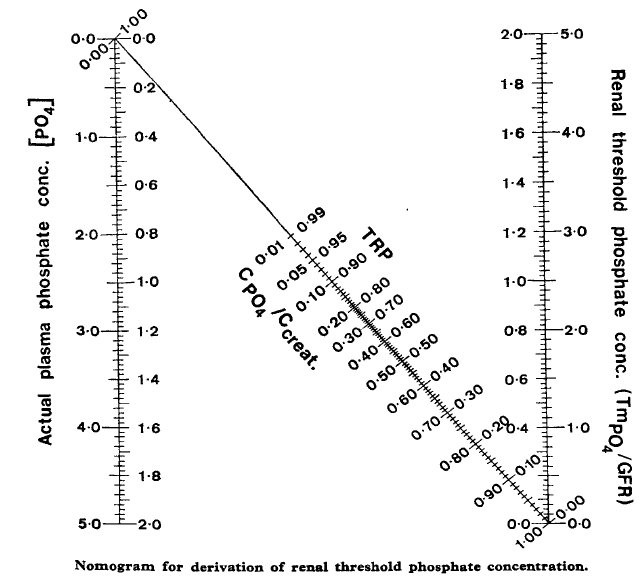
\includegraphics[scale=0.4]{nomogram.png}
				\caption{Walton and Bijvoet nomogram}
			\end{figure}
		\end{center}
\end{frame} 
%----------------------------------------------------------------------------------
\begin{frame}{How to calculate TmP/GFR?  }
	Step 1 - Calculate TRP
	\begin{block}{TRP}
		\begin{equation}
		1-\dfrac{Urine _{P}}{Urine _{Cr}} / \dfrac{Serum _{P}}{Serum _{Cr}}
		\end{equation}
	\end{block}
 Step 2 Calculate TmP/GFR
 \begin{block}{TmP/GFR}
 	\begin{equation}
 		TmP/GFR =TRP \times Serum _{P}  
 	\end{equation}
 	If TRP $ > 0.86 $
 	\begin{equation}
 	TmP/GFR =[0.3 \times TRP/(1- (0.8 \times TRP))] \times Serum _{P}
 	\end{equation}
 \end{block}
\end{frame}  
%----------------------------------------------------------------------------------
\begin{frame}{Calculating TmP/GFR  }
	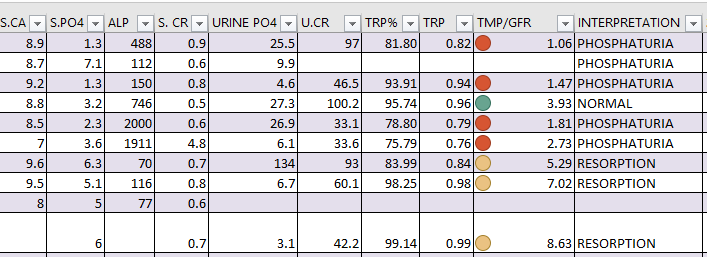
\includegraphics[width=\textwidth]{excel.png}
\end{frame}  
%---------------------------------------------------------------------------------- 
\begin{frame} {Urinalysis}
\begin{center}
		\begin{tabular}{p{4cm}p{3.5cm}l}
			\toprule
			Parameter   & Baseline  & Reference \\ \midrule
			pH          & 6.5       & 4.8 -8    \\
			Glucose     & 4+        & Nil       \\
			Aminoacids  & Positive  & Variable  \\
			Ca/Cr ratio & 0.12      & $<$ 0.2   \\
			TMP/GFR     & \myred{1.3} & 2.5-4.2   \\ \bottomrule
		\end{tabular}
\end{center}
\end{frame}
%%%%%%%%%%%%%%%%%%%%%%%%%%%%%%%%%
%---------------------------------------------------------------------------------- 


%%%%%%%%%%%%%%%%%%%%%%%%%%%%%%%%%
\begin{frame} {Bone Scan}
\begin{center}
\begin{figure}
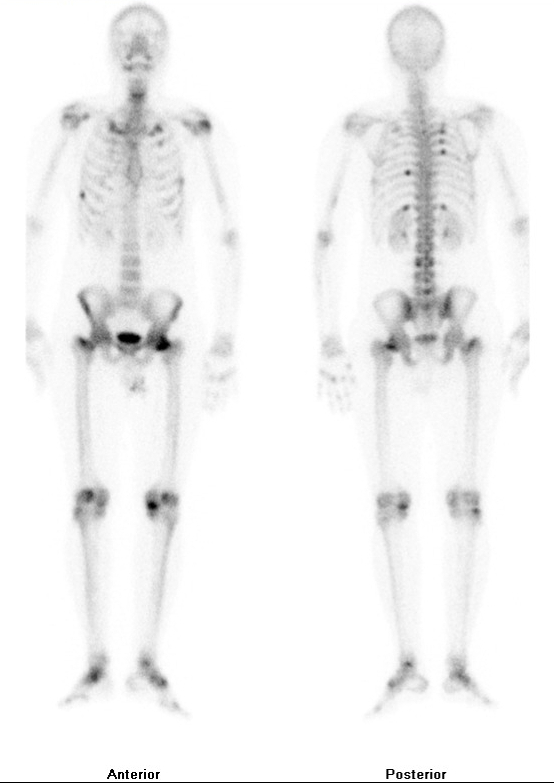
\includegraphics[height=0.7\textheight]{wholebody}
    \caption{\tiny Multiple Pseudofractures}
\end{figure}	
\end{center}	
\end{frame}
%%%%%%%%%%%%%%%%%%%%%%%%%%%%%%%%%
\begin{frame} {Description}
	\begin{itemize}
		\item Hypophosphatemic osteomalacia
        \item Proximal tubular dysfunction
\end{itemize} 
\hspace{10pt} $\oint$ Under evaluation \ldots
\end{frame}


%%%%%%%%%%%%%%%%%%%%%%%%%%%%%%%%%
\begin{frame}{Differential Diagnosis\footfullcite{Imel.2012}}
	\begin{center}
		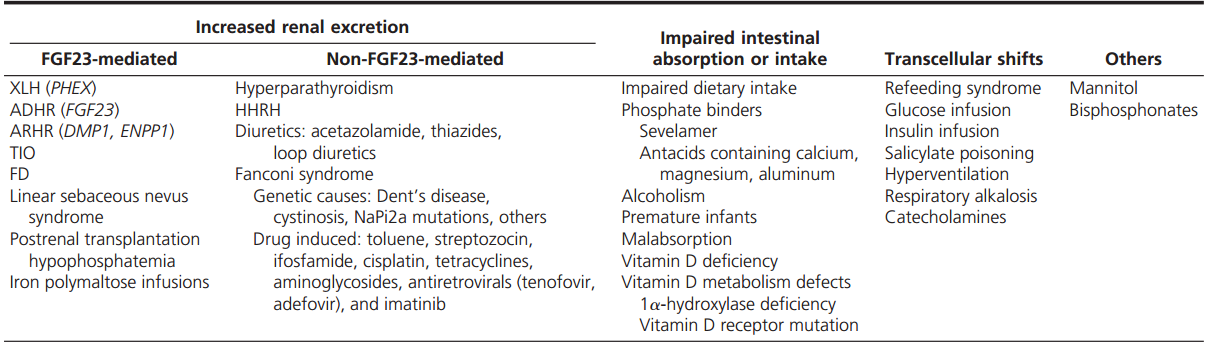
\includegraphics[width =\textwidth]{hypophosphatemia.png}
\end{center}
\end{frame}
%%%%%%%%%%%%%%%%%%%%%%%%%%%%%%%%%%%%%%%%%%%%%%%%%%%%%%%%%%
\begin{frame}{FGF23}
	\begin{block}{\textbf{C-Terminal FGF23}}
		256.7 RU/ml  (Normal: 0-150 RU/ml) 
\end{block}
\medskip\begin{bclogo} [logo=\bcbombe,barre=none,noborder=true]{Remember}
	\begin{gbar} {teal}
		FGF 23 should not be sent in serum as it gets degraded.\footfullcite{Bacchetta.2012} \\
		$ \therefore FGF \ 23 \ assay \implies EDTA \ sample $
	\end{gbar}
\end{bclogo}

\end{frame}


%%%%%%%%%%%%%%%%%%%%%%%%%%%%%%%%%%%%%%%%%%%%%%%%%%%%%%%%%%%%

%%%%%%%%%%%%%%%%%%%%%%%%%%%%%%%%%%%%%%%%%%%%%%%%%%%%%%%%%%%%%%%%%
\begin{frame}{ Interpretation }
\begin{tcolorbox}[colback=teal!5!white,colframe=teal!75!black,sidebyside]
	\begin{itemize}
	\item Hypophosphatemia
	\item Phosphaturia
	\item Normal PTH
	\item Suppressed Calcitriol
	\item High FGF 23
	\end{itemize}
	\tcblower%-----------------------------------------
	\begin{itemize}
		\item Adult onset
		\item No family history
	\end{itemize}
\end{tcolorbox}
\pause
\bigskip
$ \Longrightarrow $ TIO Vs ADHR
\end{frame} 

%---------------------------------------------------------------------------------- 
\begin{frame} {History \& Examination Revisited}
	Subcutaneous nodule of size 1.5 cm in the medial aspect of left thigh
\end{frame}

%%%%%%%%%%%%%%%%%%%%%%%%%%%%%%%%%%%%%%%%%%%%%%%%%%%%%%%%%%%%%%%%%%
\begin{frame} {Wholebody blood pool imaging}
\begin{center}
	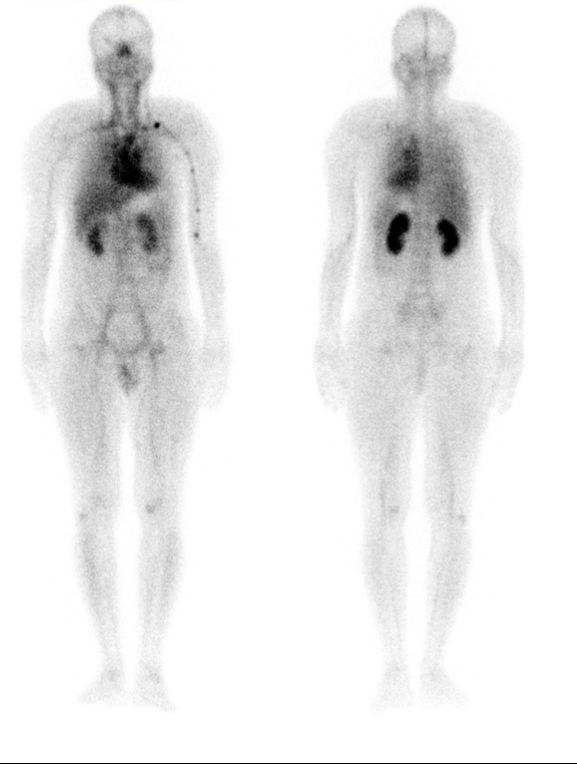
\includegraphics[scale=0.3]{bloodpool}
\end{center}
\end{frame}
%---------------------------------------------------------------------------------- 
\begin{frame}{Imaging}
	\begin{figure}
		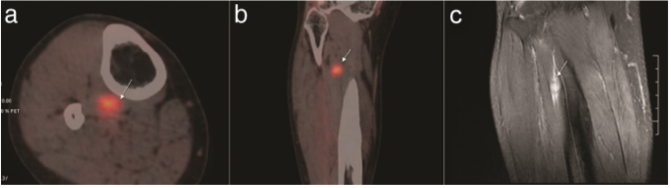
\includegraphics[scale=0.5]{fig1jcem}
       \scriptsize \caption{\textbf{a}- Fused PET-CT axial images showing FDG-avid soft tissue lesion posterolateral right proximal tibia.\\ \textbf{ b} -Fused PET-CT sagittal image of right leg showing same lesion seen on coronal section.\\ \textbf{ c} - T2 magnetic resonance coronal view shows hyperintense signal intensity right leg-SUV max : 4.86 gms/ml}
\end{figure}
\end{frame}
%%%%%%%%%%%%%%%%%%%%%%%%%%%%%%%%%%%%%%%%%%%%%%%%%%%%%%%%%%%%%%%%%%
\begin{frame}{Imaging}
\begin{center}
\begin{figure}
	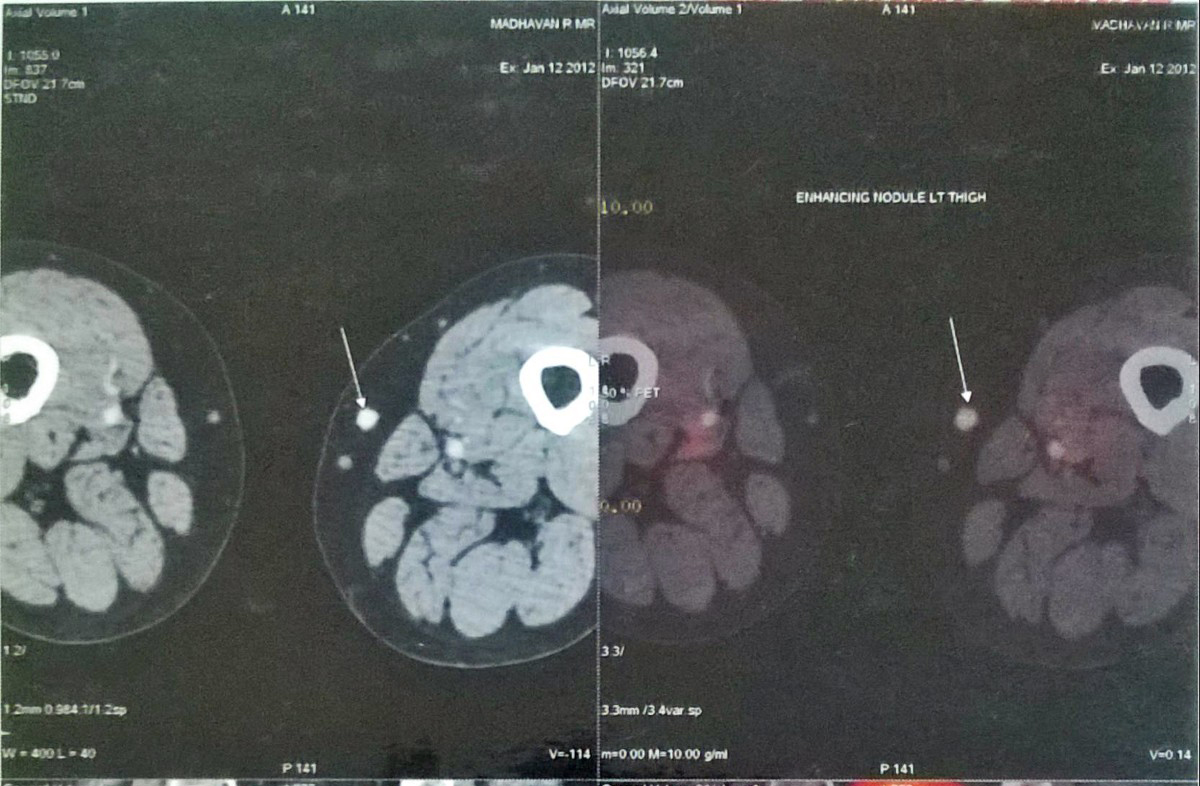
\includegraphics[scale=0.3]{thighcs}
    \caption{CT Left thigh}
\end{figure}	
\end{center}
\end{frame}
%%%%%%%%%%%%%%%%%%%%%%%%%%%%%%%%%%%%%%%%%%%%%%%%%%%%%%%%%%55%%%%5%
\begin{frame}{Imaging}
\begin{center}
\begin{figure}
	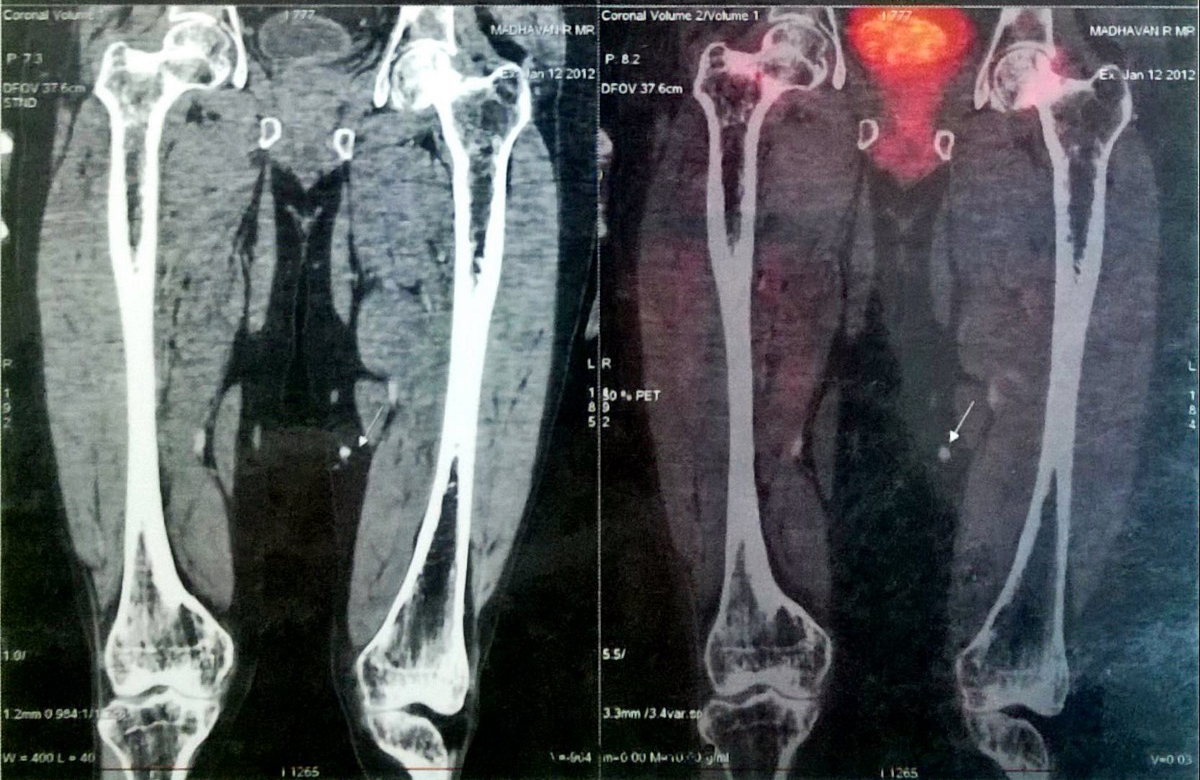
\includegraphics[scale=0.3]{thighfunc}
    \caption{PET CT(fused) Left thigh}
\end{figure}	
\end{center}
\end{frame}
%---------------------------------------------------------------------------------- 
\begin{frame}{ Imaging options \footfullcite{Jadhav.2014} }
	\begin{itemize}
		\item FDG-PET CT
		\item $ ^{99}Tc- $HYNIC-TOC SPECT CT
		\item $ ^{68} $ Ga DOTATATE 
	\end{itemize}
\end{frame}
%----------------------------------------------------------------------------------
\begin{frame}{What do we want to know?  }
\begin{block}{Conditional Probability}
  \begin{equation}
  		P(OtherScan+ | FDG -) = \dfrac{P(OtherScan+ve) \cap  P(FDG+)}{P(FDG+)}
  \end{equation}
\end{block}
\end{frame} 
%----------------------------------------------------------------------------------  
\begin{frame}{What would you do?  }
	\begin{enumerate}
         \item Remove the FDG avid lesion
         \item Remove the non FDG avid lesion
         \item Remove both
         \item Do some other scan
	\end{enumerate}
\end{frame} 

%%%%%%%%%%%%%%%%%%%%%%%%%%%%%%%%%%%%%%%%%%%%%%%%%%%%%%%%%%%%%%%%%%%%

\begin{frame}{Course}
	\begin{itemize}
		\item Patient underwent surgical excision of FDG avid lesion in the posterolateral region of right leg
        \item Post operative biochemical evaluation done
\end{itemize}
\end{frame}
%%%%%%%%%%%%%%%%%%%%%%%%%%%%%%%%%%%%%%%%%%%%%%%%%%%%%%%%%%%%%%%%%%
\begin{frame}{Biochemical parameters-Post surgery}
\begin{center}
		\begin{tabular}{p{4cm}p{3.5cm}}
			\toprule
			Parameter                 & Post Surgery \\ 
            \midrule
			Calcium                   &  7.7 mg/dl \\
			Phosphate                 & \myred{1.2 mg/dl}\\
			ALP                       & 105 IU/L \\
            TMP/GFR                   & 1.5       \\   
			\textbf{C-Terminal FGF23} & \myred{102 RU/ml}  \\
			 \bottomrule

		\end{tabular} 
\end{center}
\end{frame}
%%%%%%%%%%%%%%%%%%%%%%%%%%%%%%%%%%%%%%%%%%%%%%%%%%%%%%%%%%55%%%%5%
\begin{frame}[plain]{Histopathology}
 \begin{figure}
	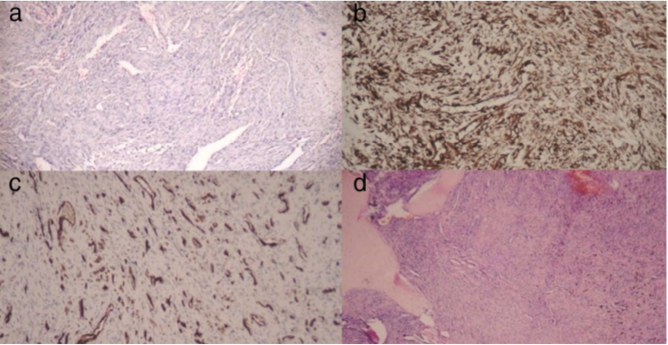
\includegraphics[scale=0.45]{fig2jcem}
    \tiny{
    	\caption{A, Proliferation of spindle cells in small fascicles and the striking
hemangiopericytomatous pattern. B, Positivity of the tumor cells for
vimentin. C, CD 34 highlighting the blood vessels and thus the
hemangiopericytomatous pattern. D, Tumor composed of spindle cells and
metaplastic osteoid formation along with focal areas showing hemosiderin-laden macrophages}
}
\end{figure}
\end{frame}
%%%%%%%%%%%%%%%%%%%%%%%%%%%%%%%%%%%%%%%%%%%%%%%%%%%%%%%%%%%%%%%%%%
\begin{frame} {Course\ldots}
	\begin{itemize}
		\item Failed first surgery in spite of complete tumor excision
        \item Waited for 8 weeks to rule out delayed remission
        \item Underwent removal of FDG negative lesion in left medial thigh
\end{itemize}
\end{frame}



%%%%%%%%%%%%%%%%%%%%%%%%%%%%%%%%%%%%%%%%%%%%%%%%%%%%%%%%%%%%%%%%%
%%%%%%%%%%%%%%%%%%%%%%%%%%%%%%%%%%%%%%%%%%%%%%%%%%%%%%%%%%%%%%%%%%
\begin{frame}{Biochemical parameters-Post surgery}
\begin{center}
		\begin{tabular}{p{4cm}p{3.5cm}l}
			\toprule
			Parameter                 & Post Surgery-1             & Post Surgery-2      \\ 
            \midrule
			Calcium                   &  7.7 mg/dl            & 9.3 mg/dl          \\
			Phosphate                 & 1.2 mg/dl            & 4.3 mg/dl        \\
			ALP                       & 105 IU/L             & 162 IU/L         \\
            TMP/GFR                   & 1.5                  & 2.4   \\   
			\textbf{C-Terminal FGF23} & \textbf{102 RU/ml} & \textbf{22 RU/ml} \\
			 \bottomrule

		\end{tabular} 
\end{center}
\end{frame}
%%%%%%%%%%%%%%%%%%%%%%%%%%%%%%%%%%%%%%%%%%%%%%%%%%%%%%%%%%%%%%%%%%
\begin{frame} {Final Diagnosis}
	\center Tumor(s) Induced Osteomalacia \footfullcite{Sahoo.2014}
\end{frame}
%%%%%%%%%%%%%%%%%%%%%%%%%%%%%%%%%%%%%%%%%%%%%%%%%%%%%%%%%%%%%%%%%%



%----------------------------------------------------------------------------------
\section{Scenarios}
\begin{frame}{I can't do FGF 23 !  }
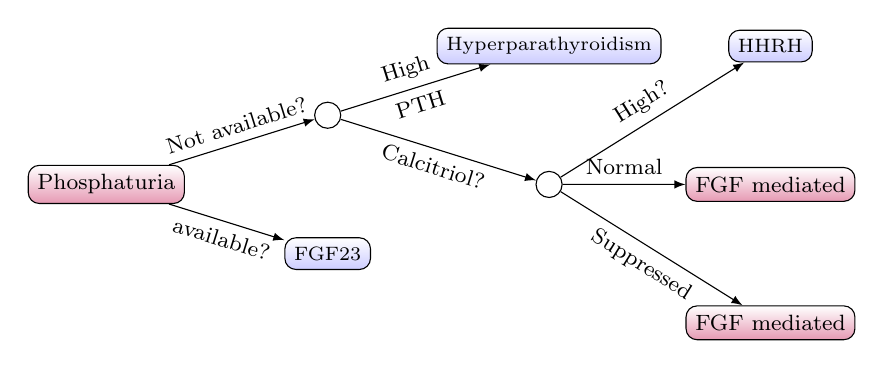
\begin{tikzpicture}
[
grow                    = right,
sibling distance        = 5em,
level distance          = 8em,
edge from parent/.style = {draw, -latex},
every node/.style       = {font=\footnotesize},
sloped
]
\node [root] {Phosphaturia}
child { node [env] {FGF23}
	edge from parent node [below] {available?} }
child { node [dummy] {}
	child { node [dummy] {}
		child { node [root] {FGF mediated}
			edge from parent node [below] {Suppressed} }
		child { node [root] {FGF mediated}
			edge from parent node [above] { Normal}
			node [below] {} }
		child { node [env] {HHRH}
			edge from parent node [above] {High?} }
		edge from parent node [below] {Calcitriol?} }
	child { node [env] {Hyperparathyroidism}
		edge from parent node [above, align=center]
		{High }
		node [below] {PTH}}
	edge from parent node [above] {Not available?} };
\end{tikzpicture}
\end{frame}
%---------------------------------------------------------------------------------- 
\begin{frame}{Tumor not found \emojicry  }
	\begin{itemize}
		\item Wait for it to show up
		\item Supplement Phosphate (40 mg/kg/day) in divided doses
		\item Give Calcitriol at 1- 3 $\mu g/day $
	\end{itemize}
\medskip
\pause
\begin{bclogo} [logo=\bcbombe,barre=none,noborder=true]{Watch out}
	\begin{itemize}
		\item Secondary hyperparathyroidism
		\item Nephrocalcinosis
	\end{itemize}
\end{bclogo}

\end{frame} 
%----------------------------------------------------------------------------------
\begin{frame}{ Tumor inoperable \emojicry }
	\begin{itemize}
		\item Radiofrequency ablation \footfullcite{Jadhav.2014}
		\begin{itemize}
			\item Close to joint
			\item Inside bone
			\item Multifocal
		\end{itemize}
		\item Octreotide
		\item Total parathyroidectomy \footfullcite{Bhadada.2013}
		\item Anti FGF 23 antibodies 
		\item PPRT
	
	\end{itemize}
\end{frame} 
%----------------------------------------------------------------------------------  
\section{Case 2} 
\begin{frame}{Case 2  }
	\begin{columns}
		\begin{column}{0.5\textwidth}
			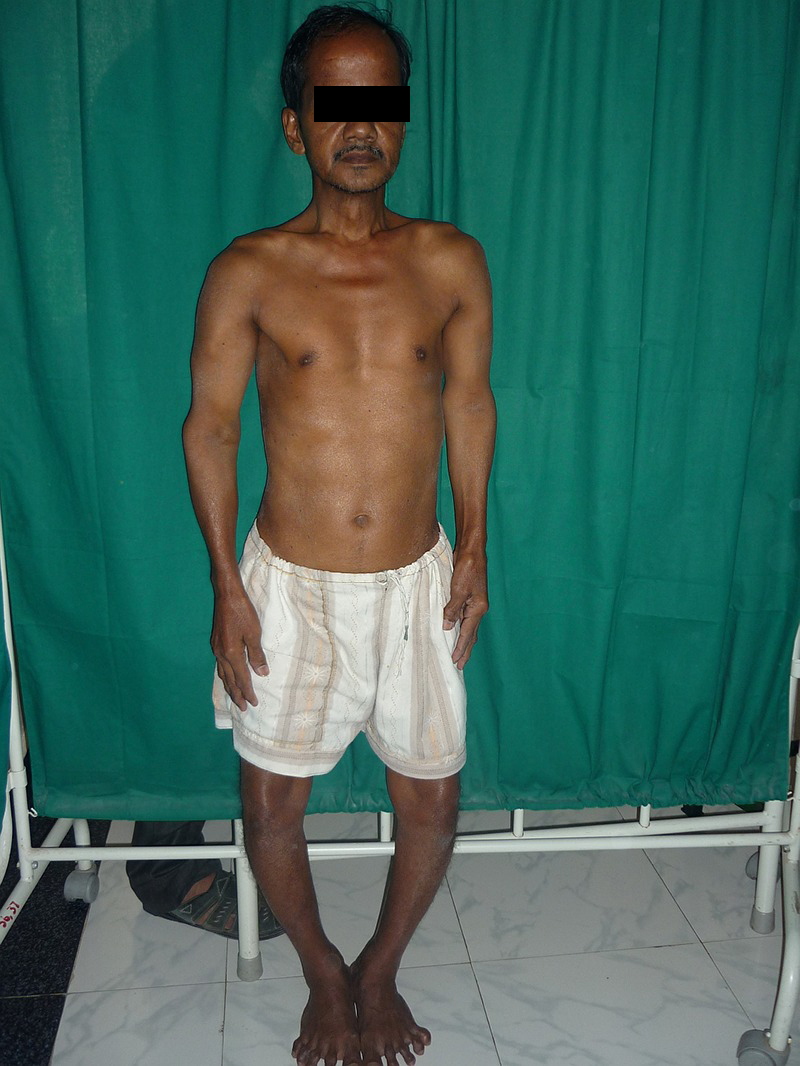
\includegraphics[scale=0.6]{case2}
		\end{column}
		
		\begin{column}{0.5\textwidth}
			\begin{itemize}
				\item Similar biochemical picture
				\item Deformities started in childhood
				\item Strong family history
				\item Dental abscess
			\end{itemize}
		\end{column}
	\end{columns}
	
\end{frame} 
%---------------------------------------------------------------------------------- 
\begin{frame}{Clinical Details  }
	\begin{figure}
		\centering
		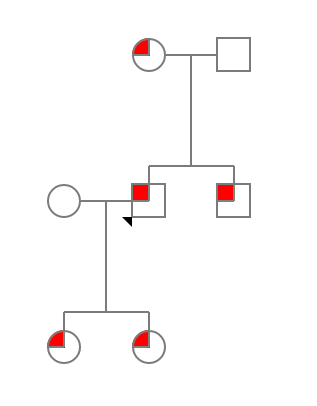
\includegraphics[height=0.7\textheight]{pedigree.png}
		\caption{Family Tree}
	\end{figure}
	
\end{frame} 
%----------------------------------------------------------------------------------
\begin{frame}{Clinical Details \footfullcite{Kumar.2015}  }
	\begin{figure}
		\centering
		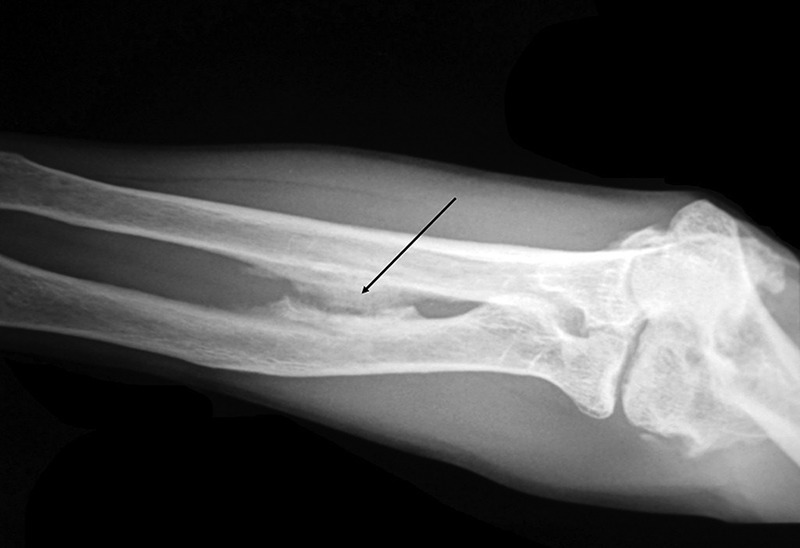
\includegraphics[width=0.7\linewidth]{osteomalacia/iom}
		\caption{Anterior interosseous membrane calcification}
		\label{fig:iom}
	\end{figure}
	
\end{frame}  
%---------------------------------------------------------------------------------- 

\begin{frame}[shrink]{Approach  }
\begin{table}[h]
	\centering
	\caption{\textit{Calcipenic vs Phosphopenic rickets}}
	\begin{tabular}{@{}lp{3.5cm}l@{}}
		\toprule
		Feature                             & Calcipenic rickets & Phosphopenic rickets   \\ \midrule
		Muscle weakness                     & Present            & Absent(except in TIO)  \\
		Bony pain                           & Common             & Uncommon               \\
		Extremities involved                & All limbs equally  & \myred{Lower limb predominant} \\
		Tetany                              & May be present     & Absent                 \\
		Enamel hypoplasia                   & May be present     & Absent                 \\
		Dental abcess                       & Absent             & \myred{May be present}         \\
		Family history                      & Less common        &  \myred{ More common}           \\
		Interosseous membrane calcification & Absent             & \myred{May be present}         \\
		Enthesopathy                        & Absent             & \myred{May be present }        \\ \bottomrule
	\end{tabular}
\end{table}
\end{frame} 
%----------------------------------------------------------------------------------
\begin{frame}{Diagnosis  }
	\center X linked Hypophosphatemic Rickets
\end{frame} 
%---------------------------------------------------------------------------------- 
\section{Conclusion}
\begin{frame}{  }
	\begin{block}{Take home}
		\begin{itemize}
			\item History,Clinical Examination and basic labs are the most important tools
			\item First principles approach and judicious use of 'fancy' investigations
			\item Multidisciplinary care is important
		\end{itemize}
	\end{block}
\end{frame} 
%----------------------------------------------------------------------------------  
\begin{frame}{ }
	\begin{center}
		\Huge {Thank You\emojismile}
	\end{center} 
\begin{textblock}{1}[0,0](0.1,0.9) 
	 \scriptsize Slides and source available \at \texttt{www.github.com/karthikjipmer}
\end{textblock}
\end{frame} 
%---------------------------------------------------------------------------------- 

\end{document}

